\documentclass[extra]{article}
%\usepackage{timet}
\usepackage[letterpaper, margin=1.5in]{geometry}
\usepackage{times}
\usepackage[round]{natbib}
\usepackage[pdftex]{graphicx}
\usepackage{amsmath}
\usepackage[obeyspaces]{url}% http://ctan.org/pkg/url
\usepackage{hyperref}% http://ctan.org/pkg/hyperref
%\usepackage{hyperref}
% delete or comment out the packages after here when submitting 
%\usepackage{lineno}
%\linenumbers
%\usepackage[disable]{todonotes}
%\usepackage{todonotes}
%\graphicspath{{./figures/}}


\begin{document}

\section{Introduction}
This document describes database and file layouts for the Seismic Hazard estimates used in the Appalachian Basin Geothermal Play Fairway Analysis \citep[GPFA-AB; ][]{GPFA-AB-Phase1FinalReport15}.  A detailed description of those techniques may be found in \citet{GPFASeismicHazardSGW15} which is an
updated version of \citet{GPFAFaultMemo15}.

\section{Details of Worms Stored in a GIS}
\label{app:WormGISDetails}
Of the techniques used in our analysis, probably the least familiar to the reader are the Poisson Wavelet Multiscale Edge Detection \citep[`worm' for brevity; ][]{WaveletTheory} results, and how they are calculated. This section describes the essence of the worm edge detection, and how those geometric objects are stored in a PostGIS database as well as reproduced here for external use.

Mathematically, the worms are calculated as points on each level of a potential fields upward continuation \citep[e.g. ][pp 313-314]{Blakely} via an edge detection procedure. Loci of points in a function \(f(x,y;z)\) that satisfy
 \begin{equation} \label{eq:EdgeDetect}
 \frac{\nabla_2 (\|\nabla_2 f\|) \cdot \nabla_2 f}{\|\nabla_2 f\|} = 0 
 \end{equation}
 are local maxima in horizontal gradients and are marked as belonging to an edge. Here, \[ \nabla_2 f \equiv (\partial/\partial x, \partial/\partial y) f \]  which is the horizontal 2D gradient vector of \(f(x,y;z)\),  and \[ \|\nabla_2 f\| \equiv  \sqrt{(\partial f/\partial x)^2 + (\partial f/\partial y)^2}\/\] which is the magnitude of that gradient vector. Strictly, points with zero horizontal gradient also satisfy equation (\ref{eq:EdgeDetect}) but they do not commonly occur in real data.
Intuitively, equation (\ref{eq:EdgeDetect}) can be thought of as describing where the gradient of the (normalized) magnitude of the gradient of \(f\) changes sign when projected along a gradient ``streamline'' of \(f\). 

Obviously, the gradients described above (and elsewhere in the processing) must be calculated in Cartesian coordinates, not in latitudes and longitudes. For the purposes of this project we performed all these calculations in UTM Zone 18N (EPSG code 32618) even though some of the data actually lie nearby in an adjacent UTM zone.  We simply accepted the relatively minor projection errors resulting from approximating one UTM zone with another for those nearby locations.

The function \(f\) in our situation is the upward-continued gravity or pseudo-gravity field from our region. 
Because \(f\) is approximated via a raster representation, we actually mark points at zero-crossings of equation (\ref{eq:EdgeDetect}) along linearly interpolated pixel boundaries -- yielding a super-resolved (sub-pixel) precision of locations for edge points.

Using freely available mathematical network/graph software \citep[NetworkX; ][]{NetworkX}, we construct a graph using the zero-crossing points identified above as graph-nodes, and connecting them via graph-edges to their nearest neighbours (identified via a spatial proximity query using kD-trees, and limited to being no further away than the diagonal length of a pixel). We then use NetworkX and custom code to construct a complete set of minimum-spanning-trees from the previously partly-organised graph data. Those minimum-spanning-trees organise our worms into distinct segments. Each segment is composed of ordered nodes that are zero-crossings of equation (\ref{eq:EdgeDetect}) and straight-line connecting edges of length no greater than the diagonal of a pixel.

Once the above data structures are computed, we store them in a working PostGIS database for retrieval by GIS software. Three interconnected tables are involved: one for the set of upward continuation levels \citep[equivalent to underground depth via the inverse wavelet transform arguments in][]{BHH01,HHB02}; one for the node points; and one for the edges. Figure \ref{fig:WormERD} displays the database tables' structure and their interconnections. Tables \ref{tab:LevelFields}, \ref{tab:PointsFields}, and \ref{tab:LevelsPointsFields} show an alternate view of the same data structures.

Open source (BSD licensed) software to perform these computations are described by \citet{HorowitzGaede14}. The \emph{git} source code management repository is located at \url{https://bitbucket.org/fghorow/bsdwormer}. By far, the easiest way to get the code running locally is to follow the directions at \url{https://bitbucket.org/fghorow/bsdwormer/wiki/Installation\%20via\%20a\%20virtual\%20machine\%20using\%20Vagrant}. 

\begin{figure}
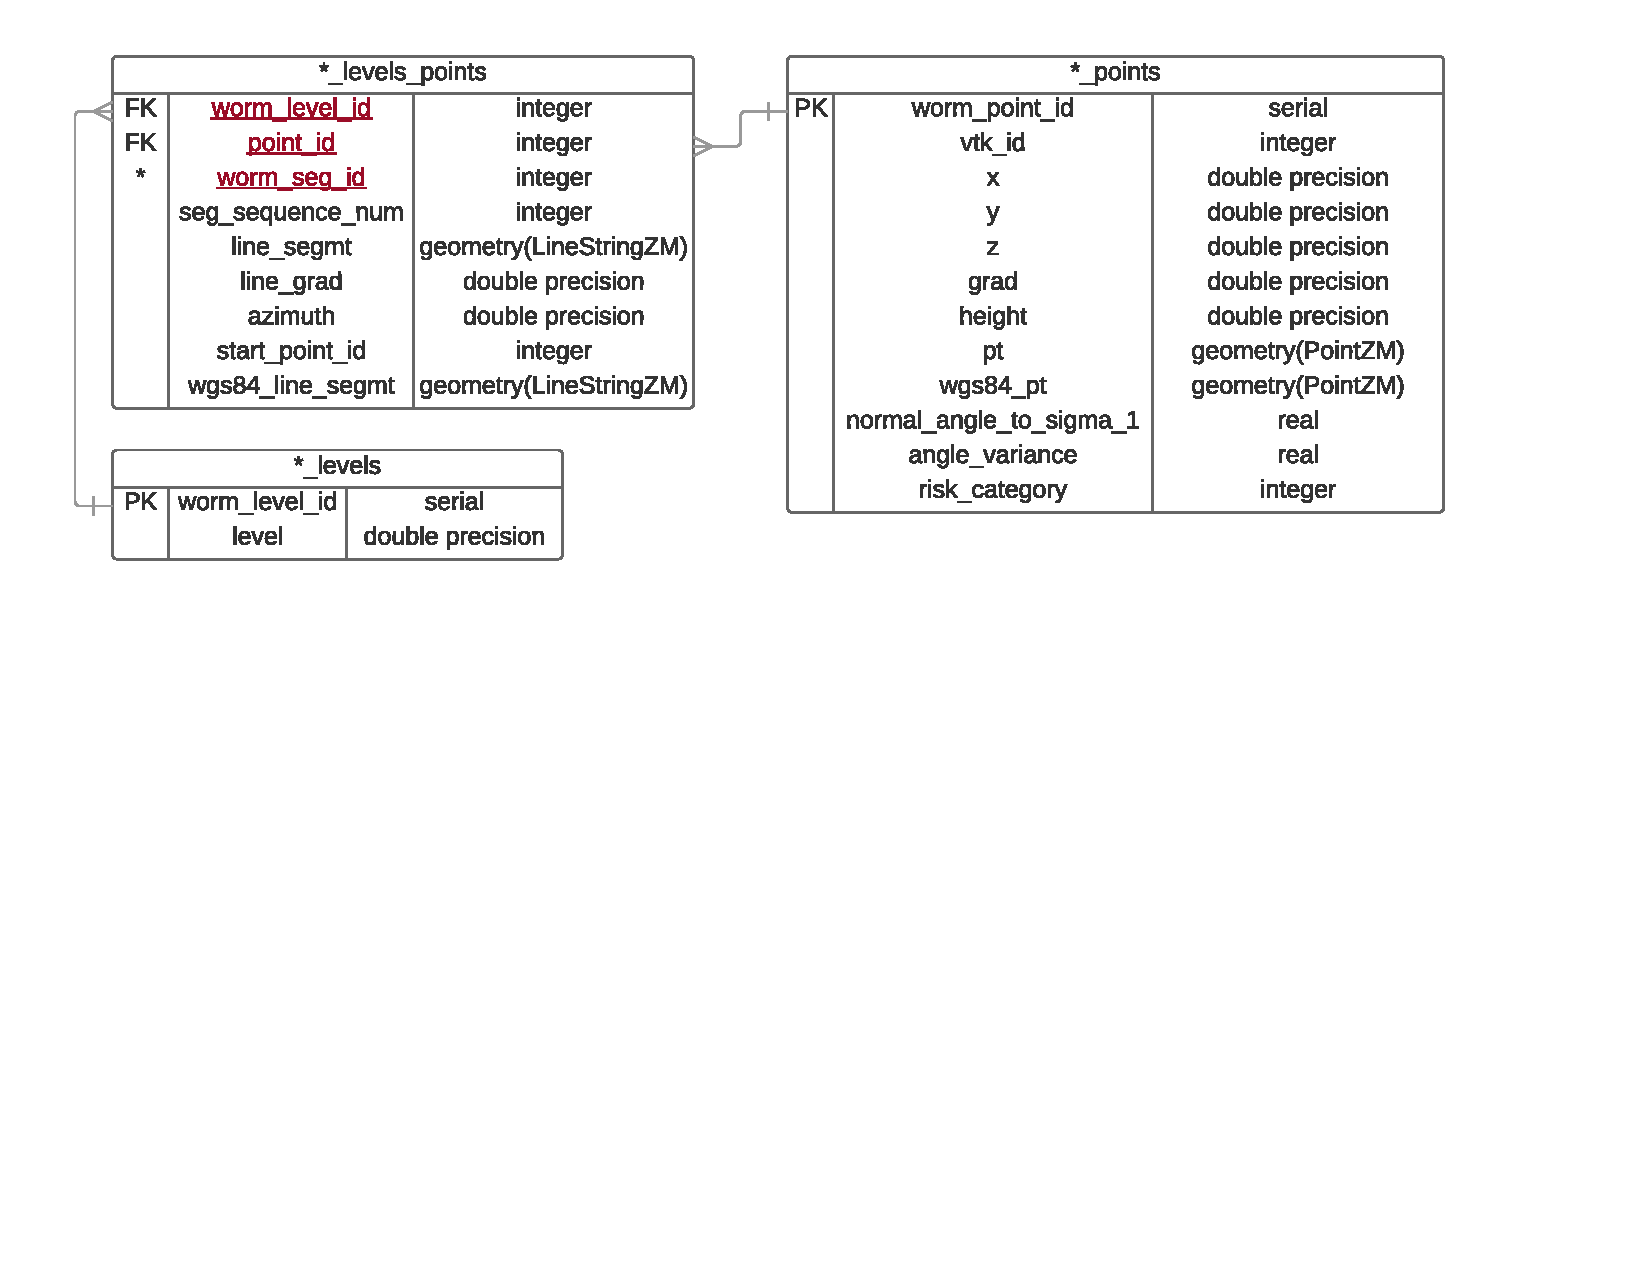
\includegraphics[width=0.90\linewidth]{WormERD.pdf}
\caption{Entity Relational Diagram for storing worms in a PostGIS database. The table labelled *\_levels holds the set of heights. The table labelled *\_points holds the points and various auxiliary attributes. The table labelled *\_levels\_points -- in addition to providing the many-to-many relationship between the other two tables -- also stores the edge's geometry as well as some attributes. This latter database table has a composite primary key (shown underlined in red) made up of pointers into the other two tables and an index `worm\_seg\_id' that enumerates the minimum-spanning-tree segments computed previously by NetworkX -- these segment-enumerating indexes are only unique within each layer, not within the database table. Within ArcGIS or QGIS, displaying either geometry field in the *\_points table shows the worm points, while displaying either geometry field in the *\_levels\_points table shows the connected worm edges.}
\label{fig:WormERD}
\end{figure}

\begin{table}[]
\centering
\caption{Description of *\_level table fields.}
\label{tab:LevelFields}
\begin{tabular}{|l|l|l|l|}
\hline
Key?        & Field Name      & Storage          & Description                              \\ \hline
Primary Key & worm\_level\_id & integer          & A unique integer: level 1, level 2, etc. \\ \hline
            & level           & double precision & Height/depth in kilometers.              \\ \hline
\end{tabular}
\end{table}

%\caption{Description of *\_level table fields.}
%\label{tab:LevelFields}

\begin{table}[]
\centering
\caption{Description of *\_points table fields.}
\label{tab:PointsFields}
\begin{tabular}{|l|l|l|l|}
\hline
Key?        & Field Name                  & Storage           & Description                                                                                                                                                                                                                                 \\ \hline
Primary Key & worm\_point\_id             & serial            & A unique integer.                                                                                                                                                                                                                           \\ \hline
            & vtk\_id                     & integer           & VTK visualization point index.                                                                                                                                                                                                              \\ \hline
            & x                           & double precision  & The UTM Eastings in meters.                                                                                                                                                                                                                 \\ \hline
            & y                           & double precision  & The UTM Northings in meters.                                                                                                                                                                                                                \\ \hline
            & z                           & double precision  & \begin{tabular}[c]{@{}l@{}}Height above/below field raster\\ in meters.\end{tabular}                                                                                                                                                        \\ \hline
            & grad                        & double precision  & \begin{tabular}[c]{@{}l@{}}The value of M in \\ (pseudo)milligals/meter.\end{tabular}                                                                                                                                                       \\ \hline
            & height                      & double precision  & \begin{tabular}[c]{@{}l@{}}Corresponds to worm\_level\_id in \\ *\_levels table.\end{tabular}                                                                                                                                               \\ \hline
            & pt                          & geometry(PointZM) & \begin{tabular}[c]{@{}l@{}}PostGIS PointZM geometry in \\ UTM18N coordinates.\end{tabular}                                                                                                                                                  \\ \hline
            & wgs84\_pt                   & geometry(PointZM) & \begin{tabular}[c]{@{}l@{}}PostGIS PointZM geometry in  WGS84 \\ coordinates. Stored for  convenience \\ of downstream processing.\end{tabular}                                                                                               \\ \hline
            & normal\_angle\_to\_sigma\_1 & real              & \begin{tabular}[c]{@{}l@{}}Angle between the normal to a \\ secant of edges at this point and the\\  World Stress Map direction of \\ principal compressive stress \\ interpolated to this location. See \\ \citet{GPFASeismicHazardSGW15} for details.\end{tabular} \\ \hline
            & angle\_variance             & real              & \begin{tabular}[c]{@{}l@{}}The variance estimate for \\ normal\_angle\_to\_sigma\_1.\\ See FIXME for details.\end{tabular}                                                                                                                  \\ \hline
            & risk\_category              & integer           & \begin{tabular}[c]{@{}l@{}}An arbitrary risk metric \\ determined by the magnitude of \\ normal\_angle\_to\_sigma\_1. \\ See text for discussion.\end{tabular}                                                                              \\ \hline
\end{tabular}
\end{table}

\begin{table}[]
\centering
\caption{Description of *\_points table fields.}
\label{tab:LevelsPointsFields}
\begin{tabular}{|l|l|l|l|}
\hline
Key?          & Field Name         & Storage                & Description                                                                                                                                                           \\ \hline
Foreign Key   & worm\_level\_id    & integer                & \begin{tabular}[c]{@{}l@{}}Pointer to worm\_level\_id in\\ the *\_levels table.\end{tabular}                                                                          \\ \hline
Foreign Key   & point\_id          & integer                & \begin{tabular}[c]{@{}l@{}}Pointer to worm\_point\_id for the end\\ point of the graph edge in the \\ *\_points table.\end{tabular}                                   \\ \hline
Composite     & worm\_seg\_id      & integer                & \begin{tabular}[c]{@{}l@{}}Identifier for connected graph edges, \\ as determined by NetworkX's\\ minimum spanning tree algorithm.\end{tabular}                       \\ \hline
              & seg\_sequence\_num & integer                & \begin{tabular}[c]{@{}l@{}}Index that orders graph edges within\\ the same worm\_seg\_id.\end{tabular}                                                                \\ \hline
              & line\_segmt        & geometry(LineStringZM) & \begin{tabular}[c]{@{}l@{}}PostGIS LineStringZM geometry for \\ each graph edge in UTM18N coordinates.\end{tabular}                                                   \\ \hline
              & line\_grad         & double precision       & \begin{tabular}[c]{@{}l@{}}The value of M averaged between \\ the values for point\_id and start\_point\_id\\ in (pseudo)milligals/meter.\end{tabular}                \\ \hline
              & Azimuth            & double precision       & \begin{tabular}[c]{@{}l@{}}Orientation of the graph edge in degrees\\ East of North.\end{tabular}                                                                     \\ \hline
(Foreign Key) & start\_point\_id   & integer                & \begin{tabular}[c]{@{}l@{}}Pointer to worm\_point\_id for the start\\ point of the graph edge in the *\_points table.\end{tabular}                                    \\ \hline
              & wgs84\_line\_segmt & geometry(LineStringZM) & \begin{tabular}[c]{@{}l@{}}PostGIS LineStringZM geometry for each\\ graph edge in WGS84 coordinates. Stored \\ for convenience of downstream processing.\end{tabular} \\ \hline
\end{tabular}
\end{table}


PostGIS databases require an appropriately configured Postgres server to be useful. Also, the interrelations between the GIS information sources shown in figure \ref{fig:WormERD} are not preserved upon export to the ArcGIS shapefile format commonly used for GIS data interchange -- due to limitations apparently inherent in the design of shapefiles. For these reasons, we chose to use a spatialite file \citep[a spatial extension to the sqlite single-file database storage format;][]{Spatialite2015} as an interchange format that preserves all of the interrelations between our database tables. Modern versions of  ArcGIS and QGIS (and hopefully other GIS systems) can read, display, and manipulate spatialite database files on an equal footing with other spatial databases, and so by this strategy we gain portability for our worm databases.

\section{Files}

These files contain the final worm results, and some of their critical upstream intermediate processing results from \citet{GPFA-AB-Phase1FinalReport15} \citep[as detailed in][]{GPFASeismicHazardSGW15, GPFAFaultMemo15}.

\begin{description}

\item[Files in the Gravity Folder] These are the gravity grids and worms for the region. 
\begin{description}
\item [GravStationsMerged.\{shp,dbf,prj,shx\}] A collection of shapefile parts containing the locations and Bouguer anomaly estimates for the measurements underlying the above interpolated grids. The Bouguer readings are in milligals, and the positions are in units of meters in the UTM zone 18N coordinate system.

\item [AppBasinMergedBGA2500.tif] This is a geotiff \citep[see, e.g. ][]{GDAL} of floating point values of the Bouguer anomaly interpolated for our study area. Pixel size is 2.5 km.
\item [AppBasinMergedBGA2500Padded.tif] This is a geotiff of the file immediately above, padded and apodized for 2D spatial Fourier transform operations. 
\item [bga\_worms.sqlite] This is a Spatialite \citep{Spatialite2015} file containing the Bouguer gravity worms in the format described in the previous section.
\item[BGAWorms.sql] This is a file of sql commands for the spatialite system \citep{Spatialite2015} that retrieves all of the interconnected Bouguer worm tables from a PostGIS database and creates the .sqlite file above. Uses the ``mod\_virtualpg'' sqlite extension (found at \url{https://www.gaia-gis.it/fossil/virtualpg/index}). Included here for reference. 

\end{description}

\item [Files in the Magnetic Folder] These are the magnetic grids and worms for the region.
\begin{description}
\item [ravat\_NURE-NAMAM2008\_UTM18N\_AppBasin.tif] A total magnetic intensity map of the region; extracted from \citet{RavatEtAl09}. In geotiff format.
\item [ravat\_NURE-NAMAM2008\_UTM18N\_AppBasin\_PSG.tif] A pseudogravity transform \citep[ see, eg.][pp. 343ff]{Blakely} of the above file. Computed using the commercial software package Oasis montaj \url{http://www.geosoft.com/products/oasis-montaj/overview}.
\item [ravat\_NURE-NAMAM2008\_UTM18N\_AppBasin\_padded\_PSG.tif] This is a geotiff of the file immediately above, padded and apodized for 2D spatial Fourier transform operations. 
\item [ravat\_mag\_worms.sqlite] This is a Spatialite \citep{Spatialite2015} file containing the  pseudogravity worms in the format described in the previous section.
\item[PSGWorms.sql] This is a file of sql commands for the spatialite system \citep{Spatialite2015} that retrieves all of the interconnected pseudogravity worm tables from a PostGIS database and creates the .sqlite file above. Uses the ``mod\_virtualpg'' sqlite extension (found at \url{https://www.gaia-gis.it/fossil/virtualpg/index}). Included here for reference. 
\end{description}


\item[Files in the Earthquakes folder] These are the recorded seismic events occurring in our study region. They are presented here in multiple forms. 
\begin{description}
\item [earthquakes.\{shp,dbf,prj,shx\}] A collection of shapefile parts containing the locations and other attributes of the earthquake hypocenters used in this work.
\item[earthquakes.\{csv,xlsx\}] The same data in both Excel spreadsheet and csv formats.
\item[SeismicHypocenters.xls] The same information as above in the spreadsheet format requested by the GDR and NGDS. 
\end{description}

\item[Files in the WorldStressMap folder] These are the observations and smoothed results from \citet{WSMDatabase08,HeidbachEtAl10}. 
\begin{description}
\item[wsm2008.xls] The authors \citep{WSMDatabase08} request that this primary spreadsheet is only to be distributed from their website. Please obtain the raw spreadsheet from there.
\item[wsm2008.sql] Data from the raw spreadsheet above have been translated into a PostGIS database for use in this project. This file contains the PostGIS SQL statements to re-create that database.
\item[wsm2008\_smoothed.\{csv,zip\}] The smoothed \(\sigma_1 \ (SH_{max})\) directions from the algorithm described in \citet{HeidbachEtAl10}. The authors request that these data too only be downloaded from the \citet{WSMDatabase08} website.
\item[DOEOrientationInStressField.ipynb] A Jupyter \citep[formerly IPython: ][]{PerezGranger07} notebook. The code for evaluating the smoothing algorithm of \citet{HeidbachEtAl10} at each node of a worm is contained in this notebook. Some standard Python 2.x libraries are required, as well as the interface library between Python and the GIS representation of the worms \citep[found in the git repository: ][]{WormDBStuff}.
\end{description}
\item[Files in the top-level folder]. These are the \LaTeX files and their intermediates for generating this README.pdf file.
\end{description}




\bibliographystyle{plainnat}
%\bibliography{fghorow}
\documentclass[extra]{article}
%\usepackage{timet}
\usepackage[letterpaper, margin=1.5in]{geometry}
\usepackage{times}
\usepackage[round]{natbib}
\usepackage[pdftex]{graphicx}
\usepackage{amsmath}
\usepackage[obeyspaces]{url}% http://ctan.org/pkg/url
\usepackage{hyperref}% http://ctan.org/pkg/hyperref
%\usepackage{hyperref}
% delete or comment out the packages after here when submitting 
%\usepackage{lineno}
%\linenumbers
%\usepackage[disable]{todonotes}
%\usepackage{todonotes}
%\graphicspath{{./figures/}}


\begin{document}

\section{Introduction}
This document describes database and file layouts for the Seismic Hazard estimates used in the Appalachian Basin Geothermal Play Fairway Analysis \citep[GPFA-AB; ][]{GPFA-AB-Phase1FinalReport15}.  A detailed description of those techniques may be found in \citet{GPFASeismicHazardSGW15} which is an
updated version of \citet{GPFAFaultMemo15}.

\section{Details of Worms Stored in a GIS}
\label{app:WormGISDetails}
Of the techniques used in our analysis, probably the least familiar to the reader are the Poisson Wavelet Multiscale Edge Detection \citep[`worm' for brevity; ][]{WaveletTheory} results, and how they are calculated. This section describes the essence of the worm edge detection, and how those geometric objects are stored in a PostGIS database as well as reproduced here for external use.

Mathematically, the worms are calculated as points on each level of a potential fields upward continuation \citep[e.g. ][pp 313-314]{Blakely} via an edge detection procedure. Loci of points in a function \(f(x,y;z)\) that satisfy
 \begin{equation} \label{eq:EdgeDetect}
 \frac{\nabla_2 (\|\nabla_2 f\|) \cdot \nabla_2 f}{\|\nabla_2 f\|} = 0 
 \end{equation}
 are local maxima in horizontal gradients and are marked as belonging to an edge. Here, \[ \nabla_2 f \equiv (\partial/\partial x, \partial/\partial y) f \]  which is the horizontal 2D gradient vector of \(f(x,y;z)\),  and \[ \|\nabla_2 f\| \equiv  \sqrt{(\partial f/\partial x)^2 + (\partial f/\partial y)^2}\/\] which is the magnitude of that gradient vector. Strictly, points with zero horizontal gradient also satisfy equation (\ref{eq:EdgeDetect}) but they do not commonly occur in real data.
Intuitively, equation (\ref{eq:EdgeDetect}) can be thought of as describing where the gradient of the (normalized) magnitude of the gradient of \(f\) changes sign when projected along a gradient ``streamline'' of \(f\). 

Obviously, the gradients described above (and elsewhere in the processing) must be calculated in Cartesian coordinates, not in latitudes and longitudes. For the purposes of this project we performed all these calculations in UTM Zone 18N (EPSG code 32618) even though some of the data actually lie nearby in an adjacent UTM zone.  We simply accepted the relatively minor projection errors resulting from approximating one UTM zone with another for those nearby locations.

The function \(f\) in our situation is the upward-continued gravity or pseudo-gravity field from our region. 
Because \(f\) is approximated via a raster representation, we actually mark points at zero-crossings of equation (\ref{eq:EdgeDetect}) along linearly interpolated pixel boundaries -- yielding a super-resolved (sub-pixel) precision of locations for edge points.

Using freely available mathematical network/graph software \citep[NetworkX; ][]{NetworkX}, we construct a graph using the zero-crossing points identified above as graph-nodes, and connecting them via graph-edges to their nearest neighbours (identified via a spatial proximity query using kD-trees, and limited to being no further away than the diagonal length of a pixel). We then use NetworkX and custom code to construct a complete set of minimum-spanning-trees from the previously partly-organised graph data. Those minimum-spanning-trees organise our worms into distinct segments. Each segment is composed of ordered nodes that are zero-crossings of equation (\ref{eq:EdgeDetect}) and straight-line connecting edges of length no greater than the diagonal of a pixel.

Once the above data structures are computed, we store them in a working PostGIS database for retrieval by GIS software. Three interconnected tables are involved: one for the set of upward continuation levels \citep[equivalent to underground depth via the inverse wavelet transform arguments in][]{BHH01,HHB02}; one for the node points; and one for the edges. Figure \ref{fig:WormERD} displays the database tables' structure and their interconnections. Tables \ref{tab:LevelFields}, \ref{tab:PointsFields}, and \ref{tab:LevelsPointsFields} show an alternate view of the same data structures.

Open source (BSD licensed) software to perform these computations are described by \citet{HorowitzGaede14}. The \emph{git} source code management repository is located at \url{https://bitbucket.org/fghorow/bsdwormer}. By far, the easiest way to get the code running locally is to follow the directions at \url{https://bitbucket.org/fghorow/bsdwormer/wiki/Installation\%20via\%20a\%20virtual\%20machine\%20using\%20Vagrant}. 

\begin{figure}
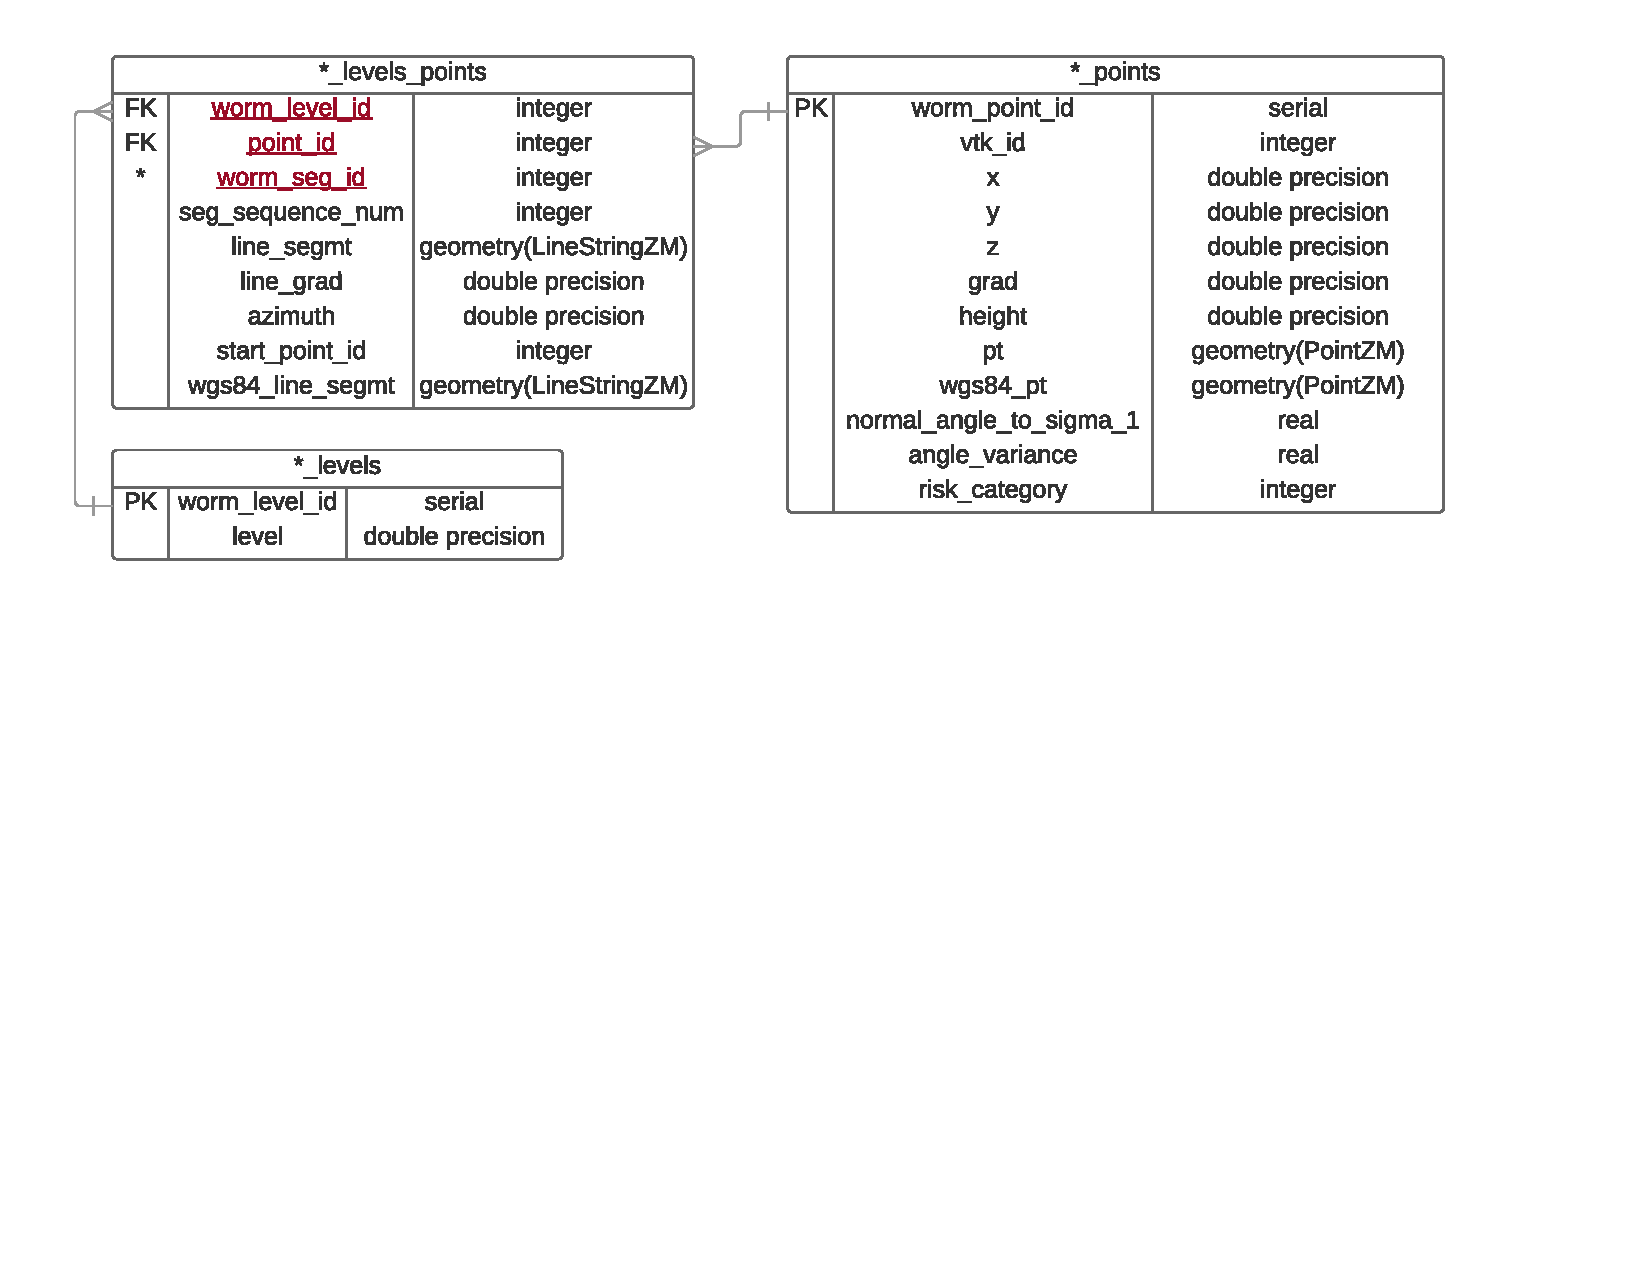
\includegraphics[width=0.90\linewidth]{WormERD.pdf}
\caption{Entity Relational Diagram for storing worms in a PostGIS database. The table labelled *\_levels holds the set of heights. The table labelled *\_points holds the points and various auxiliary attributes. The table labelled *\_levels\_points -- in addition to providing the many-to-many relationship between the other two tables -- also stores the edge's geometry as well as some attributes. This latter database table has a composite primary key (shown underlined in red) made up of pointers into the other two tables and an index `worm\_seg\_id' that enumerates the minimum-spanning-tree segments computed previously by NetworkX -- these segment-enumerating indexes are only unique within each layer, not within the database table. Within ArcGIS or QGIS, displaying either geometry field in the *\_points table shows the worm points, while displaying either geometry field in the *\_levels\_points table shows the connected worm edges.}
\label{fig:WormERD}
\end{figure}

\begin{table}[]
\centering
\caption{Description of *\_level table fields.}
\label{tab:LevelFields}
\begin{tabular}{|l|l|l|l|}
\hline
Key?        & Field Name      & Storage          & Description                              \\ \hline
Primary Key & worm\_level\_id & integer          & A unique integer: level 1, level 2, etc. \\ \hline
            & level           & double precision & Height/depth in kilometers.              \\ \hline
\end{tabular}
\end{table}

%\caption{Description of *\_level table fields.}
%\label{tab:LevelFields}

\begin{table}[]
\centering
\caption{Description of *\_points table fields.}
\label{tab:PointsFields}
\begin{tabular}{|l|l|l|l|}
\hline
Key?        & Field Name                  & Storage           & Description                                                                                                                                                                                                                                 \\ \hline
Primary Key & worm\_point\_id             & serial            & A unique integer.                                                                                                                                                                                                                           \\ \hline
            & vtk\_id                     & integer           & VTK visualization point index.                                                                                                                                                                                                              \\ \hline
            & x                           & double precision  & The UTM Eastings in meters.                                                                                                                                                                                                                 \\ \hline
            & y                           & double precision  & The UTM Northings in meters.                                                                                                                                                                                                                \\ \hline
            & z                           & double precision  & \begin{tabular}[c]{@{}l@{}}Height above/below field raster\\ in meters.\end{tabular}                                                                                                                                                        \\ \hline
            & grad                        & double precision  & \begin{tabular}[c]{@{}l@{}}The value of M in \\ (pseudo)milligals/meter.\end{tabular}                                                                                                                                                       \\ \hline
            & height                      & double precision  & \begin{tabular}[c]{@{}l@{}}Corresponds to worm\_level\_id in \\ *\_levels table.\end{tabular}                                                                                                                                               \\ \hline
            & pt                          & geometry(PointZM) & \begin{tabular}[c]{@{}l@{}}PostGIS PointZM geometry in \\ UTM18N coordinates.\end{tabular}                                                                                                                                                  \\ \hline
            & wgs84\_pt                   & geometry(PointZM) & \begin{tabular}[c]{@{}l@{}}PostGIS PointZM geometry in  WGS84 \\ coordinates. Stored for  convenience \\ of downstream processing.\end{tabular}                                                                                               \\ \hline
            & normal\_angle\_to\_sigma\_1 & real              & \begin{tabular}[c]{@{}l@{}}Angle between the normal to a \\ secant of edges at this point and the\\  World Stress Map direction of \\ principal compressive stress \\ interpolated to this location. See \\ \citet{GPFASeismicHazardSGW15} for details.\end{tabular} \\ \hline
            & angle\_variance             & real              & \begin{tabular}[c]{@{}l@{}}The variance estimate for \\ normal\_angle\_to\_sigma\_1.\\ See FIXME for details.\end{tabular}                                                                                                                  \\ \hline
            & risk\_category              & integer           & \begin{tabular}[c]{@{}l@{}}An arbitrary risk metric \\ determined by the magnitude of \\ normal\_angle\_to\_sigma\_1. \\ See text for discussion.\end{tabular}                                                                              \\ \hline
\end{tabular}
\end{table}

\begin{table}[]
\centering
\caption{Description of *\_points table fields.}
\label{tab:LevelsPointsFields}
\begin{tabular}{|l|l|l|l|}
\hline
Key?          & Field Name         & Storage                & Description                                                                                                                                                           \\ \hline
Foreign Key   & worm\_level\_id    & integer                & \begin{tabular}[c]{@{}l@{}}Pointer to worm\_level\_id in\\ the *\_levels table.\end{tabular}                                                                          \\ \hline
Foreign Key   & point\_id          & integer                & \begin{tabular}[c]{@{}l@{}}Pointer to worm\_point\_id for the end\\ point of the graph edge in the \\ *\_points table.\end{tabular}                                   \\ \hline
Composite     & worm\_seg\_id      & integer                & \begin{tabular}[c]{@{}l@{}}Identifier for connected graph edges, \\ as determined by NetworkX's\\ minimum spanning tree algorithm.\end{tabular}                       \\ \hline
              & seg\_sequence\_num & integer                & \begin{tabular}[c]{@{}l@{}}Index that orders graph edges within\\ the same worm\_seg\_id.\end{tabular}                                                                \\ \hline
              & line\_segmt        & geometry(LineStringZM) & \begin{tabular}[c]{@{}l@{}}PostGIS LineStringZM geometry for \\ each graph edge in UTM18N coordinates.\end{tabular}                                                   \\ \hline
              & line\_grad         & double precision       & \begin{tabular}[c]{@{}l@{}}The value of M averaged between \\ the values for point\_id and start\_point\_id\\ in (pseudo)milligals/meter.\end{tabular}                \\ \hline
              & Azimuth            & double precision       & \begin{tabular}[c]{@{}l@{}}Orientation of the graph edge in degrees\\ East of North.\end{tabular}                                                                     \\ \hline
(Foreign Key) & start\_point\_id   & integer                & \begin{tabular}[c]{@{}l@{}}Pointer to worm\_point\_id for the start\\ point of the graph edge in the *\_points table.\end{tabular}                                    \\ \hline
              & wgs84\_line\_segmt & geometry(LineStringZM) & \begin{tabular}[c]{@{}l@{}}PostGIS LineStringZM geometry for each\\ graph edge in WGS84 coordinates. Stored \\ for convenience of downstream processing.\end{tabular} \\ \hline
\end{tabular}
\end{table}


PostGIS databases require an appropriately configured Postgres server to be useful. Also, the interrelations between the GIS information sources shown in figure \ref{fig:WormERD} are not preserved upon export to the ArcGIS shapefile format commonly used for GIS data interchange -- due to limitations apparently inherent in the design of shapefiles. For these reasons, we chose to use a spatialite file \citep[a spatial extension to the sqlite single-file database storage format;][]{Spatialite2015} as an interchange format that preserves all of the interrelations between our database tables. Modern versions of  ArcGIS and QGIS (and hopefully other GIS systems) can read, display, and manipulate spatialite database files on an equal footing with other spatial databases, and so by this strategy we gain portability for our worm databases.

\section{Files}

These files contain the final worm results, and some of their critical upstream intermediate processing results from \citet{GPFA-AB-Phase1FinalReport15} \citep[as detailed in][]{GPFASeismicHazardSGW15, GPFAFaultMemo15}.

\begin{description}

\item[Files in the Gravity Folder] These are the gravity grids and worms for the region. 
\begin{description}
\item [GravStationsMerged.\{shp,dbf,prj,shx\}] A collection of shapefile parts containing the locations and Bouguer anomaly estimates for the measurements underlying the above interpolated grids. The Bouguer readings are in milligals, and the positions are in units of meters in the UTM zone 18N coordinate system.

\item [AppBasinMergedBGA2500.tif] This is a geotiff \citep[see, e.g. ][]{GDAL} of floating point values of the Bouguer anomaly interpolated for our study area. Pixel size is 2.5 km.
\item [AppBasinMergedBGA2500Padded.tif] This is a geotiff of the file immediately above, padded and apodized for 2D spatial Fourier transform operations. 
\item [bga\_worms.sqlite] This is a Spatialite \citep{Spatialite2015} file containing the Bouguer gravity worms in the format described in the previous section.
\item[BGAWorms.sql] This is a file of sql commands for the spatialite system \citep{Spatialite2015} that retrieves all of the interconnected Bouguer worm tables from a PostGIS database and creates the .sqlite file above. Uses the ``mod\_virtualpg'' sqlite extension (found at \url{https://www.gaia-gis.it/fossil/virtualpg/index}). Included here for reference. 

\end{description}

\item [Files in the Magnetic Folder] These are the magnetic grids and worms for the region.
\begin{description}
\item [ravat\_NURE-NAMAM2008\_UTM18N\_AppBasin.tif] A total magnetic intensity map of the region; extracted from \citet{RavatEtAl09}. In geotiff format.
\item [ravat\_NURE-NAMAM2008\_UTM18N\_AppBasin\_PSG.tif] A pseudogravity transform \citep[ see, eg.][pp. 343ff]{Blakely} of the above file. Computed using the commercial software package Oasis montaj \url{http://www.geosoft.com/products/oasis-montaj/overview}.
\item [ravat\_NURE-NAMAM2008\_UTM18N\_AppBasin\_padded\_PSG.tif] This is a geotiff of the file immediately above, padded and apodized for 2D spatial Fourier transform operations. 
\item [ravat\_mag\_worms.sqlite] This is a Spatialite \citep{Spatialite2015} file containing the  pseudogravity worms in the format described in the previous section.
\item[PSGWorms.sql] This is a file of sql commands for the spatialite system \citep{Spatialite2015} that retrieves all of the interconnected pseudogravity worm tables from a PostGIS database and creates the .sqlite file above. Uses the ``mod\_virtualpg'' sqlite extension (found at \url{https://www.gaia-gis.it/fossil/virtualpg/index}). Included here for reference. 
\end{description}


\item[Files in the Earthquakes folder] These are the recorded seismic events occurring in our study region. They are presented here in multiple forms. 
\begin{description}
\item [earthquakes.\{shp,dbf,prj,shx\}] A collection of shapefile parts containing the locations and other attributes of the earthquake hypocenters used in this work.
\item[earthquakes.\{csv,xlsx\}] The same data in both Excel spreadsheet and csv formats.
\item[SeismicHypocenters.xls] The same information as above in the spreadsheet format requested by the GDR and NGDS. 
\end{description}

\item[Files in the WorldStressMap folder] These are the observations and smoothed results from \citet{WSMDatabase08,HeidbachEtAl10}. 
\begin{description}
\item[wsm2008.xls] The authors \citep{WSMDatabase08} request that this primary spreadsheet is only to be distributed from their website. Please obtain the raw spreadsheet from there.
\item[wsm2008.sql] Data from the raw spreadsheet above have been translated into a PostGIS database for use in this project. This file contains the PostGIS SQL statements to re-create that database.
\item[wsm2008\_smoothed.\{csv,zip\}] The smoothed \(\sigma_1 \ (SH_{max})\) directions from the algorithm described in \citet{HeidbachEtAl10}. The authors request that these data too only be downloaded from the \citet{WSMDatabase08} website.
\item[DOEOrientationInStressField.ipynb] A Jupyter \citep[formerly IPython: ][]{PerezGranger07} notebook. The code for evaluating the smoothing algorithm of \citet{HeidbachEtAl10} at each node of a worm is contained in this notebook. Some standard Python 2.x libraries are required, as well as the interface library between Python and the GIS representation of the worms \citep[found in the git repository: ][]{WormDBStuff}.
\end{description}
\item[Files in the top-level folder]. These are the \LaTeX files and their intermediates for generating this README.pdf file.
\end{description}




\bibliographystyle{plainnat}
%\bibliography{fghorow}
\documentclass[extra]{article}
%\usepackage{timet}
\usepackage[letterpaper, margin=1.5in]{geometry}
\usepackage{times}
\usepackage[round]{natbib}
\usepackage[pdftex]{graphicx}
\usepackage{amsmath}
\usepackage[obeyspaces]{url}% http://ctan.org/pkg/url
\usepackage{hyperref}% http://ctan.org/pkg/hyperref
%\usepackage{hyperref}
% delete or comment out the packages after here when submitting 
%\usepackage{lineno}
%\linenumbers
%\usepackage[disable]{todonotes}
%\usepackage{todonotes}
%\graphicspath{{./figures/}}


\begin{document}

\section{Introduction}
This document describes database and file layouts for the Seismic Hazard estimates used in the Appalachian Basin Geothermal Play Fairway Analysis \citep[GPFA-AB; ][]{GPFA-AB-Phase1FinalReport15}.  A detailed description of those techniques may be found in \citet{GPFASeismicHazardSGW15} which is an
updated version of \citet{GPFAFaultMemo15}.

\section{Details of Worms Stored in a GIS}
\label{app:WormGISDetails}
Of the techniques used in our analysis, probably the least familiar to the reader are the Poisson Wavelet Multiscale Edge Detection \citep[`worm' for brevity; ][]{WaveletTheory} results, and how they are calculated. This section describes the essence of the worm edge detection, and how those geometric objects are stored in a PostGIS database as well as reproduced here for external use.

Mathematically, the worms are calculated as points on each level of a potential fields upward continuation \citep[e.g. ][pp 313-314]{Blakely} via an edge detection procedure. Loci of points in a function \(f(x,y;z)\) that satisfy
 \begin{equation} \label{eq:EdgeDetect}
 \frac{\nabla_2 (\|\nabla_2 f\|) \cdot \nabla_2 f}{\|\nabla_2 f\|} = 0 
 \end{equation}
 are local maxima in horizontal gradients and are marked as belonging to an edge. Here, \[ \nabla_2 f \equiv (\partial/\partial x, \partial/\partial y) f \]  which is the horizontal 2D gradient vector of \(f(x,y;z)\),  and \[ \|\nabla_2 f\| \equiv  \sqrt{(\partial f/\partial x)^2 + (\partial f/\partial y)^2}\/\] which is the magnitude of that gradient vector. Strictly, points with zero horizontal gradient also satisfy equation (\ref{eq:EdgeDetect}) but they do not commonly occur in real data.
Intuitively, equation (\ref{eq:EdgeDetect}) can be thought of as describing where the gradient of the (normalized) magnitude of the gradient of \(f\) changes sign when projected along a gradient ``streamline'' of \(f\). 

Obviously, the gradients described above (and elsewhere in the processing) must be calculated in Cartesian coordinates, not in latitudes and longitudes. For the purposes of this project we performed all these calculations in UTM Zone 18N (EPSG code 32618) even though some of the data actually lie nearby in an adjacent UTM zone.  We simply accepted the relatively minor projection errors resulting from approximating one UTM zone with another for those nearby locations.

The function \(f\) in our situation is the upward-continued gravity or pseudo-gravity field from our region. 
Because \(f\) is approximated via a raster representation, we actually mark points at zero-crossings of equation (\ref{eq:EdgeDetect}) along linearly interpolated pixel boundaries -- yielding a super-resolved (sub-pixel) precision of locations for edge points.

Using freely available mathematical network/graph software \citep[NetworkX; ][]{NetworkX}, we construct a graph using the zero-crossing points identified above as graph-nodes, and connecting them via graph-edges to their nearest neighbours (identified via a spatial proximity query using kD-trees, and limited to being no further away than the diagonal length of a pixel). We then use NetworkX and custom code to construct a complete set of minimum-spanning-trees from the previously partly-organised graph data. Those minimum-spanning-trees organise our worms into distinct segments. Each segment is composed of ordered nodes that are zero-crossings of equation (\ref{eq:EdgeDetect}) and straight-line connecting edges of length no greater than the diagonal of a pixel.

Once the above data structures are computed, we store them in a working PostGIS database for retrieval by GIS software. Three interconnected tables are involved: one for the set of upward continuation levels \citep[equivalent to underground depth via the inverse wavelet transform arguments in][]{BHH01,HHB02}; one for the node points; and one for the edges. Figure \ref{fig:WormERD} displays the database tables' structure and their interconnections. Tables \ref{tab:LevelFields}, \ref{tab:PointsFields}, and \ref{tab:LevelsPointsFields} show an alternate view of the same data structures.

Open source (BSD licensed) software to perform these computations are described by \citet{HorowitzGaede14}. The \emph{git} source code management repository is located at \url{https://bitbucket.org/fghorow/bsdwormer}. By far, the easiest way to get the code running locally is to follow the directions at \url{https://bitbucket.org/fghorow/bsdwormer/wiki/Installation\%20via\%20a\%20virtual\%20machine\%20using\%20Vagrant}. 

\begin{figure}
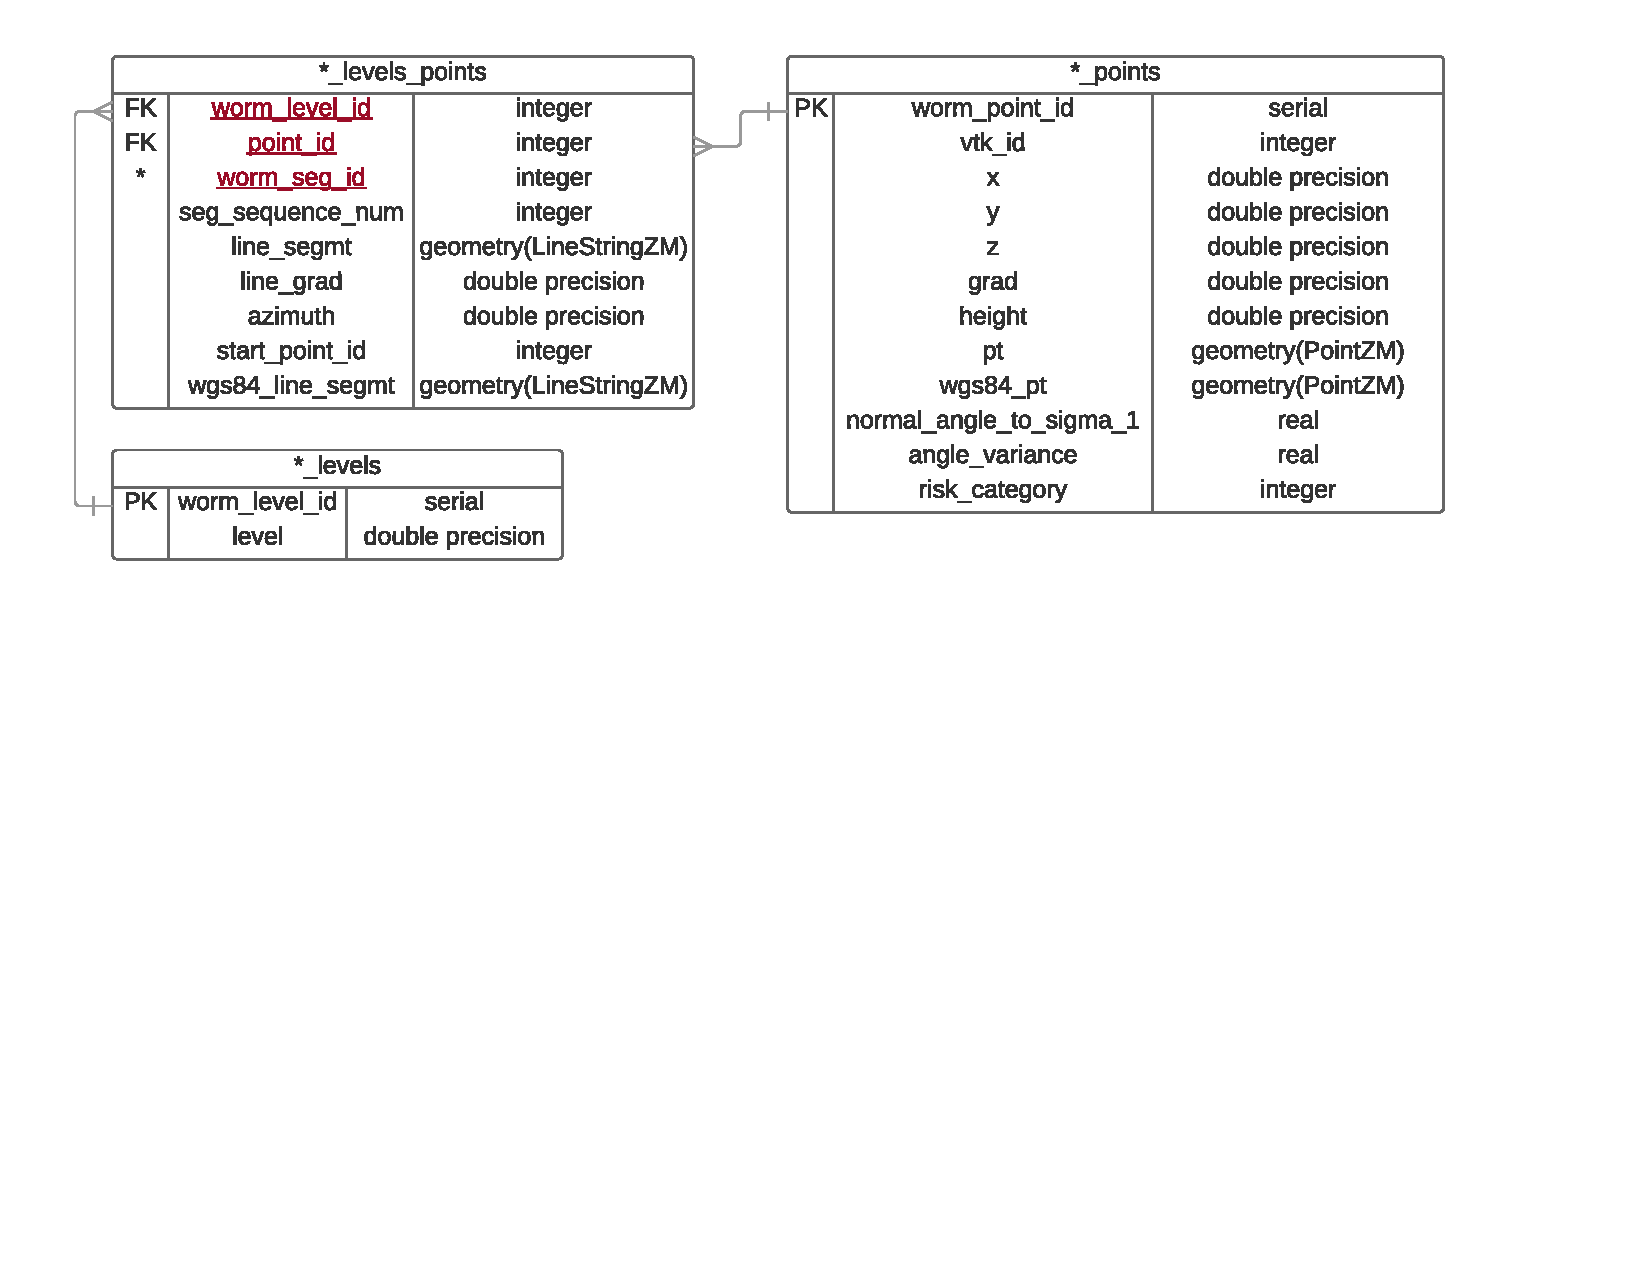
\includegraphics[width=0.90\linewidth]{WormERD.pdf}
\caption{Entity Relational Diagram for storing worms in a PostGIS database. The table labelled *\_levels holds the set of heights. The table labelled *\_points holds the points and various auxiliary attributes. The table labelled *\_levels\_points -- in addition to providing the many-to-many relationship between the other two tables -- also stores the edge's geometry as well as some attributes. This latter database table has a composite primary key (shown underlined in red) made up of pointers into the other two tables and an index `worm\_seg\_id' that enumerates the minimum-spanning-tree segments computed previously by NetworkX -- these segment-enumerating indexes are only unique within each layer, not within the database table. Within ArcGIS or QGIS, displaying either geometry field in the *\_points table shows the worm points, while displaying either geometry field in the *\_levels\_points table shows the connected worm edges.}
\label{fig:WormERD}
\end{figure}

\begin{table}[]
\centering
\caption{Description of *\_level table fields.}
\label{tab:LevelFields}
\begin{tabular}{|l|l|l|l|}
\hline
Key?        & Field Name      & Storage          & Description                              \\ \hline
Primary Key & worm\_level\_id & integer          & A unique integer: level 1, level 2, etc. \\ \hline
            & level           & double precision & Height/depth in kilometers.              \\ \hline
\end{tabular}
\end{table}

%\caption{Description of *\_level table fields.}
%\label{tab:LevelFields}

\begin{table}[]
\centering
\caption{Description of *\_points table fields.}
\label{tab:PointsFields}
\begin{tabular}{|l|l|l|l|}
\hline
Key?        & Field Name                  & Storage           & Description                                                                                                                                                                                                                                 \\ \hline
Primary Key & worm\_point\_id             & serial            & A unique integer.                                                                                                                                                                                                                           \\ \hline
            & vtk\_id                     & integer           & VTK visualization point index.                                                                                                                                                                                                              \\ \hline
            & x                           & double precision  & The UTM Eastings in meters.                                                                                                                                                                                                                 \\ \hline
            & y                           & double precision  & The UTM Northings in meters.                                                                                                                                                                                                                \\ \hline
            & z                           & double precision  & \begin{tabular}[c]{@{}l@{}}Height above/below field raster\\ in meters.\end{tabular}                                                                                                                                                        \\ \hline
            & grad                        & double precision  & \begin{tabular}[c]{@{}l@{}}The value of M in \\ (pseudo)milligals/meter.\end{tabular}                                                                                                                                                       \\ \hline
            & height                      & double precision  & \begin{tabular}[c]{@{}l@{}}Corresponds to worm\_level\_id in \\ *\_levels table.\end{tabular}                                                                                                                                               \\ \hline
            & pt                          & geometry(PointZM) & \begin{tabular}[c]{@{}l@{}}PostGIS PointZM geometry in \\ UTM18N coordinates.\end{tabular}                                                                                                                                                  \\ \hline
            & wgs84\_pt                   & geometry(PointZM) & \begin{tabular}[c]{@{}l@{}}PostGIS PointZM geometry in  WGS84 \\ coordinates. Stored for  convenience \\ of downstream processing.\end{tabular}                                                                                               \\ \hline
            & normal\_angle\_to\_sigma\_1 & real              & \begin{tabular}[c]{@{}l@{}}Angle between the normal to a \\ secant of edges at this point and the\\  World Stress Map direction of \\ principal compressive stress \\ interpolated to this location. See \\ \citet{GPFASeismicHazardSGW15} for details.\end{tabular} \\ \hline
            & angle\_variance             & real              & \begin{tabular}[c]{@{}l@{}}The variance estimate for \\ normal\_angle\_to\_sigma\_1.\\ See FIXME for details.\end{tabular}                                                                                                                  \\ \hline
            & risk\_category              & integer           & \begin{tabular}[c]{@{}l@{}}An arbitrary risk metric \\ determined by the magnitude of \\ normal\_angle\_to\_sigma\_1. \\ See text for discussion.\end{tabular}                                                                              \\ \hline
\end{tabular}
\end{table}

\begin{table}[]
\centering
\caption{Description of *\_points table fields.}
\label{tab:LevelsPointsFields}
\begin{tabular}{|l|l|l|l|}
\hline
Key?          & Field Name         & Storage                & Description                                                                                                                                                           \\ \hline
Foreign Key   & worm\_level\_id    & integer                & \begin{tabular}[c]{@{}l@{}}Pointer to worm\_level\_id in\\ the *\_levels table.\end{tabular}                                                                          \\ \hline
Foreign Key   & point\_id          & integer                & \begin{tabular}[c]{@{}l@{}}Pointer to worm\_point\_id for the end\\ point of the graph edge in the \\ *\_points table.\end{tabular}                                   \\ \hline
Composite     & worm\_seg\_id      & integer                & \begin{tabular}[c]{@{}l@{}}Identifier for connected graph edges, \\ as determined by NetworkX's\\ minimum spanning tree algorithm.\end{tabular}                       \\ \hline
              & seg\_sequence\_num & integer                & \begin{tabular}[c]{@{}l@{}}Index that orders graph edges within\\ the same worm\_seg\_id.\end{tabular}                                                                \\ \hline
              & line\_segmt        & geometry(LineStringZM) & \begin{tabular}[c]{@{}l@{}}PostGIS LineStringZM geometry for \\ each graph edge in UTM18N coordinates.\end{tabular}                                                   \\ \hline
              & line\_grad         & double precision       & \begin{tabular}[c]{@{}l@{}}The value of M averaged between \\ the values for point\_id and start\_point\_id\\ in (pseudo)milligals/meter.\end{tabular}                \\ \hline
              & Azimuth            & double precision       & \begin{tabular}[c]{@{}l@{}}Orientation of the graph edge in degrees\\ East of North.\end{tabular}                                                                     \\ \hline
(Foreign Key) & start\_point\_id   & integer                & \begin{tabular}[c]{@{}l@{}}Pointer to worm\_point\_id for the start\\ point of the graph edge in the *\_points table.\end{tabular}                                    \\ \hline
              & wgs84\_line\_segmt & geometry(LineStringZM) & \begin{tabular}[c]{@{}l@{}}PostGIS LineStringZM geometry for each\\ graph edge in WGS84 coordinates. Stored \\ for convenience of downstream processing.\end{tabular} \\ \hline
\end{tabular}
\end{table}


PostGIS databases require an appropriately configured Postgres server to be useful. Also, the interrelations between the GIS information sources shown in figure \ref{fig:WormERD} are not preserved upon export to the ArcGIS shapefile format commonly used for GIS data interchange -- due to limitations apparently inherent in the design of shapefiles. For these reasons, we chose to use a spatialite file \citep[a spatial extension to the sqlite single-file database storage format;][]{Spatialite2015} as an interchange format that preserves all of the interrelations between our database tables. Modern versions of  ArcGIS and QGIS (and hopefully other GIS systems) can read, display, and manipulate spatialite database files on an equal footing with other spatial databases, and so by this strategy we gain portability for our worm databases.

\section{Files}

These files contain the final worm results, and some of their critical upstream intermediate processing results from \citet{GPFA-AB-Phase1FinalReport15} \citep[as detailed in][]{GPFASeismicHazardSGW15, GPFAFaultMemo15}.

\begin{description}

\item[Files in the Gravity Folder] These are the gravity grids and worms for the region. 
\begin{description}
\item [GravStationsMerged.\{shp,dbf,prj,shx\}] A collection of shapefile parts containing the locations and Bouguer anomaly estimates for the measurements underlying the above interpolated grids. The Bouguer readings are in milligals, and the positions are in units of meters in the UTM zone 18N coordinate system.

\item [AppBasinMergedBGA2500.tif] This is a geotiff \citep[see, e.g. ][]{GDAL} of floating point values of the Bouguer anomaly interpolated for our study area. Pixel size is 2.5 km.
\item [AppBasinMergedBGA2500Padded.tif] This is a geotiff of the file immediately above, padded and apodized for 2D spatial Fourier transform operations. 
\item [bga\_worms.sqlite] This is a Spatialite \citep{Spatialite2015} file containing the Bouguer gravity worms in the format described in the previous section.
\item[BGAWorms.sql] This is a file of sql commands for the spatialite system \citep{Spatialite2015} that retrieves all of the interconnected Bouguer worm tables from a PostGIS database and creates the .sqlite file above. Uses the ``mod\_virtualpg'' sqlite extension (found at \url{https://www.gaia-gis.it/fossil/virtualpg/index}). Included here for reference. 

\end{description}

\item [Files in the Magnetic Folder] These are the magnetic grids and worms for the region.
\begin{description}
\item [ravat\_NURE-NAMAM2008\_UTM18N\_AppBasin.tif] A total magnetic intensity map of the region; extracted from \citet{RavatEtAl09}. In geotiff format.
\item [ravat\_NURE-NAMAM2008\_UTM18N\_AppBasin\_PSG.tif] A pseudogravity transform \citep[ see, eg.][pp. 343ff]{Blakely} of the above file. Computed using the commercial software package Oasis montaj \url{http://www.geosoft.com/products/oasis-montaj/overview}.
\item [ravat\_NURE-NAMAM2008\_UTM18N\_AppBasin\_padded\_PSG.tif] This is a geotiff of the file immediately above, padded and apodized for 2D spatial Fourier transform operations. 
\item [ravat\_mag\_worms.sqlite] This is a Spatialite \citep{Spatialite2015} file containing the  pseudogravity worms in the format described in the previous section.
\item[PSGWorms.sql] This is a file of sql commands for the spatialite system \citep{Spatialite2015} that retrieves all of the interconnected pseudogravity worm tables from a PostGIS database and creates the .sqlite file above. Uses the ``mod\_virtualpg'' sqlite extension (found at \url{https://www.gaia-gis.it/fossil/virtualpg/index}). Included here for reference. 
\end{description}


\item[Files in the Earthquakes folder] These are the recorded seismic events occurring in our study region. They are presented here in multiple forms. 
\begin{description}
\item [earthquakes.\{shp,dbf,prj,shx\}] A collection of shapefile parts containing the locations and other attributes of the earthquake hypocenters used in this work.
\item[earthquakes.\{csv,xlsx\}] The same data in both Excel spreadsheet and csv formats.
\item[SeismicHypocenters.xls] The same information as above in the spreadsheet format requested by the GDR and NGDS. 
\end{description}

\item[Files in the WorldStressMap folder] These are the observations and smoothed results from \citet{WSMDatabase08,HeidbachEtAl10}. 
\begin{description}
\item[wsm2008.xls] The authors \citep{WSMDatabase08} request that this primary spreadsheet is only to be distributed from their website. Please obtain the raw spreadsheet from there.
\item[wsm2008.sql] Data from the raw spreadsheet above have been translated into a PostGIS database for use in this project. This file contains the PostGIS SQL statements to re-create that database.
\item[wsm2008\_smoothed.\{csv,zip\}] The smoothed \(\sigma_1 \ (SH_{max})\) directions from the algorithm described in \citet{HeidbachEtAl10}. The authors request that these data too only be downloaded from the \citet{WSMDatabase08} website.
\item[DOEOrientationInStressField.ipynb] A Jupyter \citep[formerly IPython: ][]{PerezGranger07} notebook. The code for evaluating the smoothing algorithm of \citet{HeidbachEtAl10} at each node of a worm is contained in this notebook. Some standard Python 2.x libraries are required, as well as the interface library between Python and the GIS representation of the worms \citep[found in the git repository: ][]{WormDBStuff}.
\end{description}
\item[Files in the top-level folder]. These are the \LaTeX files and their intermediates for generating this README.pdf file.
\end{description}




\bibliographystyle{plainnat}
%\bibliography{fghorow}
\documentclass[extra]{article}
%\usepackage{timet}
\usepackage[letterpaper, margin=1.5in]{geometry}
\usepackage{times}
\usepackage[round]{natbib}
\usepackage[pdftex]{graphicx}
\usepackage{amsmath}
\usepackage[obeyspaces]{url}% http://ctan.org/pkg/url
\usepackage{hyperref}% http://ctan.org/pkg/hyperref
%\usepackage{hyperref}
% delete or comment out the packages after here when submitting 
%\usepackage{lineno}
%\linenumbers
%\usepackage[disable]{todonotes}
%\usepackage{todonotes}
%\graphicspath{{./figures/}}


\begin{document}

\section{Introduction}
This document describes database and file layouts for the Seismic Hazard estimates used in the Appalachian Basin Geothermal Play Fairway Analysis \citep[GPFA-AB; ][]{GPFA-AB-Phase1FinalReport15}.  A detailed description of those techniques may be found in \citet{GPFASeismicHazardSGW15} which is an
updated version of \citet{GPFAFaultMemo15}.

\section{Details of Worms Stored in a GIS}
\label{app:WormGISDetails}
Of the techniques used in our analysis, probably the least familiar to the reader are the Poisson Wavelet Multiscale Edge Detection \citep[`worm' for brevity; ][]{WaveletTheory} results, and how they are calculated. This section describes the essence of the worm edge detection, and how those geometric objects are stored in a PostGIS database as well as reproduced here for external use.

Mathematically, the worms are calculated as points on each level of a potential fields upward continuation \citep[e.g. ][pp 313-314]{Blakely} via an edge detection procedure. Loci of points in a function \(f(x,y;z)\) that satisfy
 \begin{equation} \label{eq:EdgeDetect}
 \frac{\nabla_2 (\|\nabla_2 f\|) \cdot \nabla_2 f}{\|\nabla_2 f\|} = 0 
 \end{equation}
 are local maxima in horizontal gradients and are marked as belonging to an edge. Here, \[ \nabla_2 f \equiv (\partial/\partial x, \partial/\partial y) f \]  which is the horizontal 2D gradient vector of \(f(x,y;z)\),  and \[ \|\nabla_2 f\| \equiv  \sqrt{(\partial f/\partial x)^2 + (\partial f/\partial y)^2}\/\] which is the magnitude of that gradient vector. Strictly, points with zero horizontal gradient also satisfy equation (\ref{eq:EdgeDetect}) but they do not commonly occur in real data.
Intuitively, equation (\ref{eq:EdgeDetect}) can be thought of as describing where the gradient of the (normalized) magnitude of the gradient of \(f\) changes sign when projected along a gradient ``streamline'' of \(f\). 

Obviously, the gradients described above (and elsewhere in the processing) must be calculated in Cartesian coordinates, not in latitudes and longitudes. For the purposes of this project we performed all these calculations in UTM Zone 18N (EPSG code 32618) even though some of the data actually lie nearby in an adjacent UTM zone.  We simply accepted the relatively minor projection errors resulting from approximating one UTM zone with another for those nearby locations.

The function \(f\) in our situation is the upward-continued gravity or pseudo-gravity field from our region. 
Because \(f\) is approximated via a raster representation, we actually mark points at zero-crossings of equation (\ref{eq:EdgeDetect}) along linearly interpolated pixel boundaries -- yielding a super-resolved (sub-pixel) precision of locations for edge points.

Using freely available mathematical network/graph software \citep[NetworkX; ][]{NetworkX}, we construct a graph using the zero-crossing points identified above as graph-nodes, and connecting them via graph-edges to their nearest neighbours (identified via a spatial proximity query using kD-trees, and limited to being no further away than the diagonal length of a pixel). We then use NetworkX and custom code to construct a complete set of minimum-spanning-trees from the previously partly-organised graph data. Those minimum-spanning-trees organise our worms into distinct segments. Each segment is composed of ordered nodes that are zero-crossings of equation (\ref{eq:EdgeDetect}) and straight-line connecting edges of length no greater than the diagonal of a pixel.

Once the above data structures are computed, we store them in a working PostGIS database for retrieval by GIS software. Three interconnected tables are involved: one for the set of upward continuation levels \citep[equivalent to underground depth via the inverse wavelet transform arguments in][]{BHH01,HHB02}; one for the node points; and one for the edges. Figure \ref{fig:WormERD} displays the database tables' structure and their interconnections. Tables \ref{tab:LevelFields}, \ref{tab:PointsFields}, and \ref{tab:LevelsPointsFields} show an alternate view of the same data structures.

Open source (BSD licensed) software to perform these computations are described by \citet{HorowitzGaede14}. The \emph{git} source code management repository is located at \url{https://bitbucket.org/fghorow/bsdwormer}. By far, the easiest way to get the code running locally is to follow the directions at \url{https://bitbucket.org/fghorow/bsdwormer/wiki/Installation\%20via\%20a\%20virtual\%20machine\%20using\%20Vagrant}. 

\begin{figure}
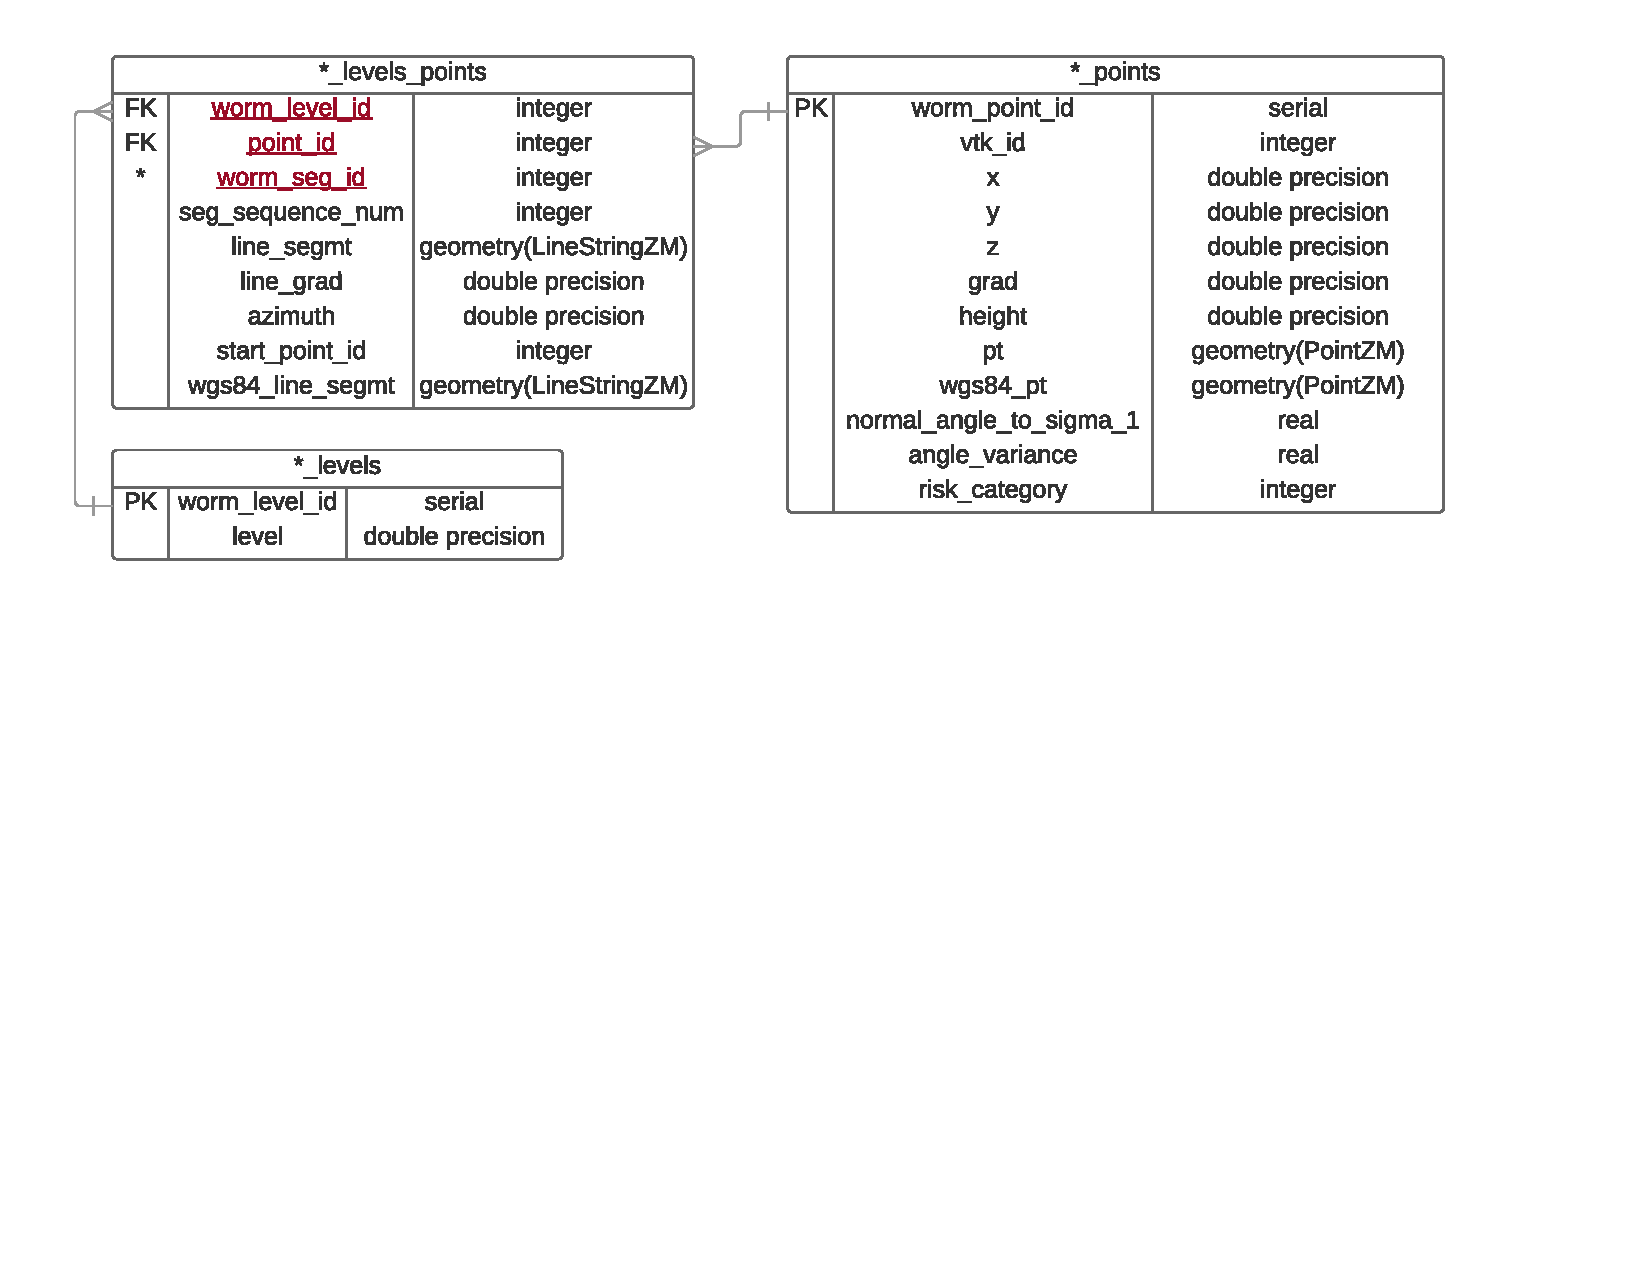
\includegraphics[width=0.90\linewidth]{WormERD.pdf}
\caption{Entity Relational Diagram for storing worms in a PostGIS database. The table labelled *\_levels holds the set of heights. The table labelled *\_points holds the points and various auxiliary attributes. The table labelled *\_levels\_points -- in addition to providing the many-to-many relationship between the other two tables -- also stores the edge's geometry as well as some attributes. This latter database table has a composite primary key (shown underlined in red) made up of pointers into the other two tables and an index `worm\_seg\_id' that enumerates the minimum-spanning-tree segments computed previously by NetworkX -- these segment-enumerating indexes are only unique within each layer, not within the database table. Within ArcGIS or QGIS, displaying either geometry field in the *\_points table shows the worm points, while displaying either geometry field in the *\_levels\_points table shows the connected worm edges.}
\label{fig:WormERD}
\end{figure}

\begin{table}[]
\centering
\caption{Description of *\_level table fields.}
\label{tab:LevelFields}
\begin{tabular}{|l|l|l|l|}
\hline
Key?        & Field Name      & Storage          & Description                              \\ \hline
Primary Key & worm\_level\_id & integer          & A unique integer: level 1, level 2, etc. \\ \hline
            & level           & double precision & Height/depth in kilometers.              \\ \hline
\end{tabular}
\end{table}

%\caption{Description of *\_level table fields.}
%\label{tab:LevelFields}

\begin{table}[]
\centering
\caption{Description of *\_points table fields.}
\label{tab:PointsFields}
\begin{tabular}{|l|l|l|l|}
\hline
Key?        & Field Name                  & Storage           & Description                                                                                                                                                                                                                                 \\ \hline
Primary Key & worm\_point\_id             & serial            & A unique integer.                                                                                                                                                                                                                           \\ \hline
            & vtk\_id                     & integer           & VTK visualization point index.                                                                                                                                                                                                              \\ \hline
            & x                           & double precision  & The UTM Eastings in meters.                                                                                                                                                                                                                 \\ \hline
            & y                           & double precision  & The UTM Northings in meters.                                                                                                                                                                                                                \\ \hline
            & z                           & double precision  & \begin{tabular}[c]{@{}l@{}}Height above/below field raster\\ in meters.\end{tabular}                                                                                                                                                        \\ \hline
            & grad                        & double precision  & \begin{tabular}[c]{@{}l@{}}The value of M in \\ (pseudo)milligals/meter.\end{tabular}                                                                                                                                                       \\ \hline
            & height                      & double precision  & \begin{tabular}[c]{@{}l@{}}Corresponds to worm\_level\_id in \\ *\_levels table.\end{tabular}                                                                                                                                               \\ \hline
            & pt                          & geometry(PointZM) & \begin{tabular}[c]{@{}l@{}}PostGIS PointZM geometry in \\ UTM18N coordinates.\end{tabular}                                                                                                                                                  \\ \hline
            & wgs84\_pt                   & geometry(PointZM) & \begin{tabular}[c]{@{}l@{}}PostGIS PointZM geometry in  WGS84 \\ coordinates. Stored for  convenience \\ of downstream processing.\end{tabular}                                                                                               \\ \hline
            & normal\_angle\_to\_sigma\_1 & real              & \begin{tabular}[c]{@{}l@{}}Angle between the normal to a \\ secant of edges at this point and the\\  World Stress Map direction of \\ principal compressive stress \\ interpolated to this location. See \\ \citet{GPFASeismicHazardSGW15} for details.\end{tabular} \\ \hline
            & angle\_variance             & real              & \begin{tabular}[c]{@{}l@{}}The variance estimate for \\ normal\_angle\_to\_sigma\_1.\\ See FIXME for details.\end{tabular}                                                                                                                  \\ \hline
            & risk\_category              & integer           & \begin{tabular}[c]{@{}l@{}}An arbitrary risk metric \\ determined by the magnitude of \\ normal\_angle\_to\_sigma\_1. \\ See text for discussion.\end{tabular}                                                                              \\ \hline
\end{tabular}
\end{table}

\begin{table}[]
\centering
\caption{Description of *\_points table fields.}
\label{tab:LevelsPointsFields}
\begin{tabular}{|l|l|l|l|}
\hline
Key?          & Field Name         & Storage                & Description                                                                                                                                                           \\ \hline
Foreign Key   & worm\_level\_id    & integer                & \begin{tabular}[c]{@{}l@{}}Pointer to worm\_level\_id in\\ the *\_levels table.\end{tabular}                                                                          \\ \hline
Foreign Key   & point\_id          & integer                & \begin{tabular}[c]{@{}l@{}}Pointer to worm\_point\_id for the end\\ point of the graph edge in the \\ *\_points table.\end{tabular}                                   \\ \hline
Composite     & worm\_seg\_id      & integer                & \begin{tabular}[c]{@{}l@{}}Identifier for connected graph edges, \\ as determined by NetworkX's\\ minimum spanning tree algorithm.\end{tabular}                       \\ \hline
              & seg\_sequence\_num & integer                & \begin{tabular}[c]{@{}l@{}}Index that orders graph edges within\\ the same worm\_seg\_id.\end{tabular}                                                                \\ \hline
              & line\_segmt        & geometry(LineStringZM) & \begin{tabular}[c]{@{}l@{}}PostGIS LineStringZM geometry for \\ each graph edge in UTM18N coordinates.\end{tabular}                                                   \\ \hline
              & line\_grad         & double precision       & \begin{tabular}[c]{@{}l@{}}The value of M averaged between \\ the values for point\_id and start\_point\_id\\ in (pseudo)milligals/meter.\end{tabular}                \\ \hline
              & Azimuth            & double precision       & \begin{tabular}[c]{@{}l@{}}Orientation of the graph edge in degrees\\ East of North.\end{tabular}                                                                     \\ \hline
(Foreign Key) & start\_point\_id   & integer                & \begin{tabular}[c]{@{}l@{}}Pointer to worm\_point\_id for the start\\ point of the graph edge in the *\_points table.\end{tabular}                                    \\ \hline
              & wgs84\_line\_segmt & geometry(LineStringZM) & \begin{tabular}[c]{@{}l@{}}PostGIS LineStringZM geometry for each\\ graph edge in WGS84 coordinates. Stored \\ for convenience of downstream processing.\end{tabular} \\ \hline
\end{tabular}
\end{table}


PostGIS databases require an appropriately configured Postgres server to be useful. Also, the interrelations between the GIS information sources shown in figure \ref{fig:WormERD} are not preserved upon export to the ArcGIS shapefile format commonly used for GIS data interchange -- due to limitations apparently inherent in the design of shapefiles. For these reasons, we chose to use a spatialite file \citep[a spatial extension to the sqlite single-file database storage format;][]{Spatialite2015} as an interchange format that preserves all of the interrelations between our database tables. Modern versions of  ArcGIS and QGIS (and hopefully other GIS systems) can read, display, and manipulate spatialite database files on an equal footing with other spatial databases, and so by this strategy we gain portability for our worm databases.

\section{Files}

These files contain the final worm results, and some of their critical upstream intermediate processing results from \citet{GPFA-AB-Phase1FinalReport15} \citep[as detailed in][]{GPFASeismicHazardSGW15, GPFAFaultMemo15}.

\begin{description}

\item[Files in the Gravity Folder] These are the gravity grids and worms for the region. 
\begin{description}
\item [GravStationsMerged.\{shp,dbf,prj,shx\}] A collection of shapefile parts containing the locations and Bouguer anomaly estimates for the measurements underlying the above interpolated grids. The Bouguer readings are in milligals, and the positions are in units of meters in the UTM zone 18N coordinate system.

\item [AppBasinMergedBGA2500.tif] This is a geotiff \citep[see, e.g. ][]{GDAL} of floating point values of the Bouguer anomaly interpolated for our study area. Pixel size is 2.5 km.
\item [AppBasinMergedBGA2500Padded.tif] This is a geotiff of the file immediately above, padded and apodized for 2D spatial Fourier transform operations. 
\item [bga\_worms.sqlite] This is a Spatialite \citep{Spatialite2015} file containing the Bouguer gravity worms in the format described in the previous section.
\item[BGAWorms.sql] This is a file of sql commands for the spatialite system \citep{Spatialite2015} that retrieves all of the interconnected Bouguer worm tables from a PostGIS database and creates the .sqlite file above. Uses the ``mod\_virtualpg'' sqlite extension (found at \url{https://www.gaia-gis.it/fossil/virtualpg/index}). Included here for reference. 

\end{description}

\item [Files in the Magnetic Folder] These are the magnetic grids and worms for the region.
\begin{description}
\item [ravat\_NURE-NAMAM2008\_UTM18N\_AppBasin.tif] A total magnetic intensity map of the region; extracted from \citet{RavatEtAl09}. In geotiff format.
\item [ravat\_NURE-NAMAM2008\_UTM18N\_AppBasin\_PSG.tif] A pseudogravity transform \citep[ see, eg.][pp. 343ff]{Blakely} of the above file. Computed using the commercial software package Oasis montaj \url{http://www.geosoft.com/products/oasis-montaj/overview}.
\item [ravat\_NURE-NAMAM2008\_UTM18N\_AppBasin\_padded\_PSG.tif] This is a geotiff of the file immediately above, padded and apodized for 2D spatial Fourier transform operations. 
\item [ravat\_mag\_worms.sqlite] This is a Spatialite \citep{Spatialite2015} file containing the  pseudogravity worms in the format described in the previous section.
\item[PSGWorms.sql] This is a file of sql commands for the spatialite system \citep{Spatialite2015} that retrieves all of the interconnected pseudogravity worm tables from a PostGIS database and creates the .sqlite file above. Uses the ``mod\_virtualpg'' sqlite extension (found at \url{https://www.gaia-gis.it/fossil/virtualpg/index}). Included here for reference. 
\end{description}


\item[Files in the Earthquakes folder] These are the recorded seismic events occurring in our study region. They are presented here in multiple forms. 
\begin{description}
\item [earthquakes.\{shp,dbf,prj,shx\}] A collection of shapefile parts containing the locations and other attributes of the earthquake hypocenters used in this work.
\item[earthquakes.\{csv,xlsx\}] The same data in both Excel spreadsheet and csv formats.
\item[SeismicHypocenters.xls] The same information as above in the spreadsheet format requested by the GDR and NGDS. 
\end{description}

\item[Files in the WorldStressMap folder] These are the observations and smoothed results from \citet{WSMDatabase08,HeidbachEtAl10}. 
\begin{description}
\item[wsm2008.xls] The authors \citep{WSMDatabase08} request that this primary spreadsheet is only to be distributed from their website. Please obtain the raw spreadsheet from there.
\item[wsm2008.sql] Data from the raw spreadsheet above have been translated into a PostGIS database for use in this project. This file contains the PostGIS SQL statements to re-create that database.
\item[wsm2008\_smoothed.\{csv,zip\}] The smoothed \(\sigma_1 \ (SH_{max})\) directions from the algorithm described in \citet{HeidbachEtAl10}. The authors request that these data too only be downloaded from the \citet{WSMDatabase08} website.
\item[DOEOrientationInStressField.ipynb] A Jupyter \citep[formerly IPython: ][]{PerezGranger07} notebook. The code for evaluating the smoothing algorithm of \citet{HeidbachEtAl10} at each node of a worm is contained in this notebook. Some standard Python 2.x libraries are required, as well as the interface library between Python and the GIS representation of the worms \citep[found in the git repository: ][]{WormDBStuff}.
\end{description}
\item[Files in the top-level folder]. These are the \LaTeX files and their intermediates for generating this README.pdf file.
\end{description}




\bibliographystyle{plainnat}
%\bibliography{fghorow}
\input{README.bbl}


\end{document}



\end{document}



\end{document}



\end{document}
